\chapter{Introduction}\label{C:intro}
The Kepler Exoplanet dataset \cite{datasetphl} \cite{dataset}  contains information about planets from outside of
our solar system. This information was discovered by the Kepler space observatory, shown in Figure
\ref{fig:keplerTele}. The Kepler space observatory was launched in 2009 by NASA
to discover Earth like planets orbiting other stars \cite{keplerTele}.

\begin{figure}[H]
  \centering
      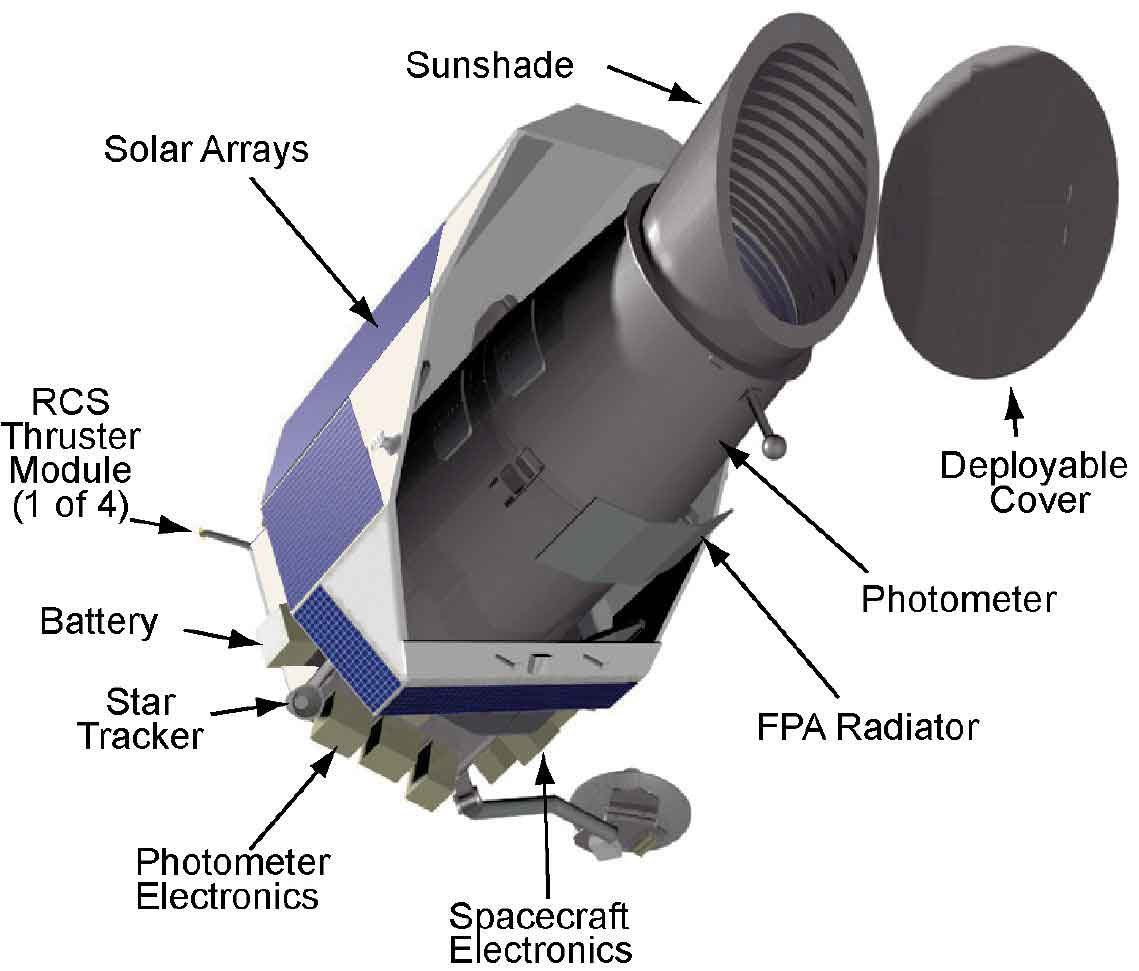
\includegraphics[width=0.8\textwidth]{images/keplerTele.jpg}
  \caption[Kepler space observatory]{A rendering of the Kepler space observatory}  
    \label{fig:keplerTele}
\end{figure}

% Introduction to the Kepler Mission 
This project seeks to design, implement, and evaluate an interactive 3D
visualisation software system for displaying the data contained in the Kepler
Exoplanet dataset using both gestures and traditional interactive methods. This deliverable is intended as a standalone
3D visualisation with two modes of interaction: keyboard \& mouse or Microsoft
Xbox Kinect sensor \cite{kinect}. The resulting visualisation will present the
information from the dataset in a way that the target users, laypeople who have
an
interest in astronomy, can understand and interact with.
\section{Problem Statement}
Many planets have been identified outside of our own solar system,
these are called exoplanets, and are referred to interchangeably as planets and
exoplanets for the remainder of this report. Information about these exoplanets
is available in the Kepler Exoplanet Dataset
. This project seeks to develop and evaluate an interactive 3D
visualisation software system for the Kepler Exoplanets Dataset. Visualisations
are valuable as they foster immersion and enjoyment, both of which result in
improved learning and recall. This means that
creating an effective and engaging visualisation will help convey the
information
in the dataset effectively to the users.

The complex nature of the information involved in this project causes a range of
problems revolving around understandability and access to the data in the dataset. This project
attempts to address these issues in a way that results in increased
accessibility of the information contained in the dataset for laypeople. The
following subsections outline these in detail.

\subsection{Understanding the Content in the Dataset}
Understanding and analysing large datasets whose size defies simplistic or
trivial analysis by humans is a known issue, and one that many areas of research
are
attempting to address. These areas of research include data mining, data
analytics, and visualisations in order to discover and highlight important
features in the data so that people can more easily understand and use it \cite{chan}. 

% Internal and External Visualisation
Humans often rely on internal visualisation to solve problems. We create an
image in our mind of a situation in order to make sense of it
 which allows for a faster and more comprehensive
understanding \cite{visualisingpiggott}. The content in the dataset used
for this project is made up of records of every one of the 2234 exoplanets
discovered by the Kepler Mission. Each of these records contains 46 fields, shown
in Figure \ref{fig:fields}, which
makes it next to impossible for someone to internally visualise as there is so
much information, especially as most of it consists of floating point numbers.
This means that an external
way of visualising the data is needed.
\begin{figure}[H]
  \centering
      
\includegraphics[width=0.8\textwidth]{images/data.png}
  \caption[Kepler Exoplanet dataset fields]{The fields of the Kepler Exoplanet dataset, the amount and variety of which makes them difficult to comprehend}
  \label{fig:fields}
\end{figure}
 This project aims to find a way to display this information visually
so that users can better understand it.
\subsection{Comprehension of Planetary Information}
Much of the information regarding planets is cryptic and unintuitive, this makes
it difficult to understand. Data visualisation can therefore be effective
because it shifts the balance between perception and cognition to take advantage
of
the brain's abilities. Seeing (i.e. visual perception) which is handled by the
visual cortex located in the rear of the brain, is extremely fast and efficient.
We see immediately, with little effort. Thinking (i.e. cognition), which is
handled primarily by the cerebral cortex in the front of the brain, is much
slower and less efficient \cite{few}. Therefore this project will find ways of
visually simplifying this data so that it conveys more meaning to users. 


\subsection{Existing Solutions Lack Functionality}
Existing data visualisations using this exoplanet dataset lack the
ability to display sufficient detail for each exoplanet and do not fully utilise
the data available. Existing solutions display only the size, temperature,
and orbital information about the exoplanets. While this is useful information
that informs users of important facts about the planets, it leaves a lot of
potentially useful information unseen and overlooked. 
Examples of this include, information about types of planet, solar system information,
planet similarities, and habitability. This project will therefore focus on
researching, implementing, and evaluating a new interactive visualisation system
that displays information contained in the dataset but not
included in existing visualisation systems.

\subsection{Effective User Interaction with Visualisation}
A visualisation that solely displays information without effective methods of
interaction limits the immersive qualities that keeps users engaged.

To address
this, interactive visualisations emerged, generally these visualisations allow
users to modify the representation of information rather than the information
itself. This means allowing users to control properties of how the data is
represented, be it something as simple as the layout of elements or
more complex. Many mediums of interaction are possible from the mundane
keyboards, mice, or touchpads to the more esoteric wired gloves, motion sensors,
and gesture recognition or even a combination of devices. Existing
visualisations surrounding planetary data only allow access to a small subset of
the information contained within the Kepler Exoplanet Database. In addition to
this most solutions do not allow interaction with any advanced means with the
exception of Exo \cite{exo} which uses wired gloves to detect the gestures of of
users. To address this this project incorporates a range of interactive
components that allow the user to access large amounts of data. It also
introduces a new novel method of interacting with the visualisation via gestures
with a Microsoft Kinect sensor.

\section{Key Issues Project Addresses}
To summarise the above sections, this project addresses the following key
issues:
\begin{description}
 \item[Issue 1.] Content in the Kepler Exoplanet Database is difficult to view
and
understand due to its amount and labeling.
 \item[Issue 2.] Planetary information is complex and difficult to comprehend
without
a visual reference due to its scale.
 \item[Issue 3.] Existing visualisations for exploring planetary data have
minimal
functionality for exploring the information in effective ways.
 \item[Issue 4.] Visualisations need to allow user interaction to make the most
of
the data they display.
\end{description}
These issues are explored in Chapter \ref{Chap:ra} to create
the project requirements.

\section{Contributions of this Project}
This project provides an interactive 3D visualisation that conveys more information and
contains better interactivity than other visualisations in the same field. This
extension is evaluated both qualitatively and quantitatively by a within subjects user experiment to ensure that it
successfully conveys the information in the Kepler Exoplanet Database.
A key part of this project is the development of interactive techniques to provide the best access to the data. These techniques are a mix of keyboard and
mouse as well as a novel gesture based approach using a Microsoft Kinect sensor.
The work and research completed for this project will provide the opportunity
for further improvement of the produced visualisation in the future.
